\documentclass[11pt]{article}
\usepackage{isma2018}

% Enter further packages required for your manuscript below.
\usepackage{graphicx}
\usepackage{caption}
\usepackage{subcaption}
%%%%%%%%%%%%%%%%%%%%%%%%%%%%%%%%%%%%%%%%%%%%%%%%%%%%%%%%%%%%%%%%%%%
% The "hyperref" package may be used in conjunction with PDFLatex %
% to add document information to the generated PDF file. Please,  %
% fill out the same title, author(s) and keywords as on the paper %
% submission form. Note, that the "hypperref" package should be   %
% loaded as the last.                                             %
%                                                                 %
% If you are not using PDFLatex, delete or comment the following  %
% lines. In that case, the conference secretary will add the      %
% document information to your PDF file.                          %
%%%%%%%%%%%%%%%%%%%%%%%%%%%%%%%%%%%%%%%%%%%%%%%%%%%%%%%%%%%%%%%%%%%

\usepackage[pdftex]{hyperref}
\hypersetup{a4paper = true,
	pdfpagemode = None,
	pdfstartview  = FitH,
	citebordercolor = 1 1 1,
	filebordercolor = 1 1 1,
	linkbordercolor = 1 1 1,
	urlbordercolor = 1 1 1}
\hypersetup{pdftitle  = {Manuscript preparation instructions},
	pdfauthor = {A. Michalak,  A. Wy{\l}oma{\'n}ska, J. Wodecki,  R. Zimroz, K. Gryllias},
	pdfkeywords = {local damage detection, vibration signal analysis, ADF test}}


\usepackage[numbers,square,sort&compress]{natbib}
\usepackage{color}


\title{Optimal frequency band selection via stationarity testing in time frequency domain}

\author{\textbf{A. Michalak $^1$,  A. Wy{\l}oma{\'n}ska $^1$, J. Wodecki $^1$,  R. Zimroz $^2$, K. Gryllias $^3$, $^4$} \\
  $^1$ Research and Development Centre, KGHM Cuprum Ltd, \\ 
  Sikorskiego 2-8, 53-659 Wroc{\l}aw, Poland  \\
  e-mail: \textbf{\{amichalak, awylomanska, jwodecki\}@cuprum.wroc.pl} 
% % Uncomment this block to add multiple (different) affiliations.
 \\ [3mm]
  $^2$ Faculty of Geoengineering, Mining and Geology, Diagnostics and Vibro-Acoustic Science Laboratory, Wroc{\l}aw University of Science and Technology,\\
  Na Grobli 15, 50-421 Wroc{\l}aw, Poland \\
  e-mail: \textbf{radoslaw.zimroz@pwr.wroc.pl} 
  \\ [3mm]
  $^3$ KU Leuven, Department of Mechanical Engineering, \\
  Celestijnenlaan 300 - box 2420, 3001 Leuven, Belgium
  \\ [3mm]
  $^4$ Dynamics of Mechanical and Mechatronic Systems, Flanders Make, Belgium\\
  e-mail: \textbf{konstantinos.gryllias@kuleuven.be} 
  }

\date{}

\begin{document}

\abstract{In the era of Industry 4.0 and smart machines, condition monitoring of rotating machinery plays an important role. In the last decades a plethora of signal processing tools have been proposed for the analysis of vibration signals, focusing towards the early and accurate fault detection and diagnosis of rotating machinery. Some of the existing algorithms are based on the filtering around an informative frequency band, which contains the diagnostic information usually in the form of a modulation of a carrier frequency by a characteristic fault frequencies. A number of approaches and experience rules have been proposed during the last decade for the optimum manual or automatic identification and selection of the informative frequency band where usually the Signal-to-Noise Ratio (SNR) is high and the fault is more easily detected. Although the existence of numerous methodologies, there is still a clear industrial need to construct more specific diagnostic algorithms, since real-life industrial signals are usually non-typical, noisy, complex and difficult to be handled. The informative frequency band is a purely frequency-domain idea, so very often the approach of spectral selectors is pursued, and those are, simply speaking, digital filters prepared in a custom way. In this paper a novel signal processing approach is proposed based on the analysis of the time-frequency domain. Following briefly the procedure, the vibration signal is firstly transformed to the time-frequency domain. Moreover, the stationarity of the time series vectors within the discrete frequency bins of the Time-Frequency (T-F) map is statistically tested by using the Augmented Dickey-Fuller (ADF) test in order to check if the given signal corresponds to a healthy or a damaged machine. A frequency band filter selector is then constructed by the aggregation of the ADF statistic values of narrow frequency bins into a vector spanning over the whole Nyquist band of the given signal.}

\maketitle

\section{Introduction}
The notion of introducing so-called \emph{intelligent solutions} for maintenance of industrial machinery drives the need for development of specialized analytical methods for more and more demanding diagnostic scenarios. Machines with rotating components are one of the most investigated types of objects due to high diversity of possible fault cases regarding components interacting with each other. Mechanisms of signal generation by kinematic pairs when one of component is faulty has been research problem studied by many researchers \cite{randall1982new,chaari2008effect,antoni2002differential,antoni2003stochastic}. Nowadays it is well known that fault signature in case of rolling element bearings or gearboxes will be impulsive \cite{antoni2006spectral}, cyclic (or periodic) \cite{michalak2017application}, nonlinear, non-Gaussian \cite{wylomanska2016application}, amplitude/phase modulated \cite{chaari2012gearbox}, etc. Most of these descriptors was already used as detection criteria - kurtosis was used as measure of impulsiveness \cite{wodecki2018optimal}, cylcostationary analysis was developed to detect and identify cycles related to damage \cite{wodecki2017informative, kruczek2017multiple} etc. However in this paper authors propose to use testing of the signal stationarity for machine diagnostics. It is well known, that in case of healthy bearings, signal measured on the housing will be stationary and closely resemble one having Gaussian distribution. In case of local damage, two surfaces in contact will produce a disturbance. Effectively, series of such impacts in time domain will manifest itself as a cyclic (or periodic) additive impulsive component. It will definitely introduce disturbance in the signal, which will contribute to the degree of non-stationarity. This observation, made already also by others is basis for this paper \cite{martin2007advanced}. A key idea here is to test whether signal is stationary or not. Although, instead of evaluating signal as of itself, authors propose more structure-oriented approach. Due to complexity of machine and number of potential sources of non-stationarity, including accidental disturbances \cite{wodecki2017local,zak2017measures}, testing of stationarity will be done in time-frequency domain, for each frequency bin -- similarly as in spectral kurtosis (SK) or other methods developed for informative frequency band identification. There are plenty of techniques for testing of stationarity of the signal \cite{dickey1979distribution,durbin1951testing,kwiatkowski1992testing}. In presented paper authors propose to use Augmented Dickey-Fuller (ADF) test \cite{dickey1979distribution}. As a result, one can obtain distribution of ADF statistic value along the frequency scale, which can be used as a spectral selector similarly to SK and it could be basis for digital filter characteristic for signal enhancement \cite{obuchowski2014selection}. This approach has been validated for real signal from pulley bearing. As a validation step, result is compared with the SK method in terms of selector shape as well as quality of obtained filtered signal.


\section{Methodology}

In this section key aspects of the methodology are described. The main idea is to develop frequency-domain selector based on the spectral stationarity of the signal. Our approach in some sense is an extension of the classical metodology based on the spectral kurtosis, popular measure of impulsiveness, however we take under consideration the ADF statistic (calculated for each frequency band) which may indicate the nonstationarity of subsignal corresponding to given frequency band.  Flowchart of proposed algorithm is presented in Figure \ref{f:block}.

\begin{figure}[!ht]
\begin{center}
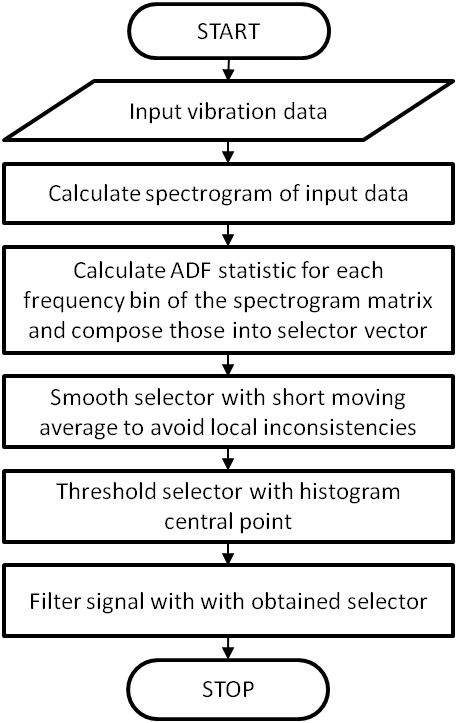
\includegraphics[width=0.5\textwidth]{block}
\caption{Flowchart of proposed procedure. \label{f:block}}
\end{center}
\end{figure}

First, spectrogram of the input data is calculated as a time-frequency representation. It allows to access narrow frequency bands. Next, for each subsignal from the time-frequency representation we calculate ADF statistic  (see Equation (\ref{eq:spec})). We should mention, the ADF test based on the ADF statistic,  is a classical one used to test nonstationarity of real data. Next, the selector is smoothed and thresholded.  In the following subsections we describe details of the proposed procedure.

\subsection{Time-frequency representation}
Presented procedure begins with calculating spectrogram (see Equations (\ref{eq:spectrogram}) and (\ref{eq:spec})). Its parameters are selected based on empirical testing and are suited best for the length of signal time series. For analyzed real signal (see section 3) the parameters are presented in Table \ref{tab:tab}.

The short-time Fourier transform (STFT) for the discrete signal $y_0, y_1, \dots , y_{N-1}$ is defined as follows \cite{oppenheim1999discrete}:
\begin{equation}
\label{eq:spectrogram}
\textrm{STFT}(t,f)=\sum_{m=0}^{L-1} y_{t+m}\omega_{m}e^{-j2\pi fm/N}
\end{equation}
for $0\leq f\leq f_{max}$ and $0\leq t\leq t_{max}$. In the above equation $\omega$ is the shifted window of the length $L$. Furthermore, the spectrogram is squared absolute value of the STFT:

\begin{equation}
\label{eq:spec}
\textrm{Spec}(t,f)=|\textrm{STFT}(t,f)|^2.
\end{equation}

\subsection{ADF selector}
The problem of testing stationarity of real data is widely discussed in the literature. One can find different approaches applied in this issue. The classical tests are for instance DF (Dikey-Fuller), KPSS (Kwiatkowski-Phillips-Schmidt-Shin) or Durbin-Watson 
\cite{dickey1979distribution,kwiatkowski1992testing,durbin1951testing}. However one of the most popular test for stationarity is the augmented Dickey–Fuller test (ADF). The null hypothesis of the ADF test is that the unit root is present in analyzed data, i.e. the data follow the model:
\begin{equation}
    \label{ADF_model}
    y_t=c+\delta t + \phi y_{t-1} + \beta _1 \Delta y_{t-1} + \dots +  \beta _p \Delta y_{t-p} + \epsilon _t,
\end{equation}
where $\Delta$ is the differencing operator, $p$ is the number of lagged difference terms and $
\{\epsilon _t\}$ constitutes a sample of independent identically Gaussian distributed random variables with mean zero and variance $\sigma^2$ $ \left( N(0,\sigma^2) \right) $. The unit root is when $\phi=1$, i.e. after differentiation the signal corresponds to autoregressive process of order $p$ (AR(p)).
In presented case authors take under consideration the simpler version with no drift ($c=0$), no trend ($\delta=0$) and (p=0). In this case the model (\ref{ADF_model}) takes the form:
\begin{equation}
    \label{ADF_model_1}
    y_t=\phi y_{t-1} + \epsilon _t,
\end{equation}
which is  autoregressive model of order 1 (AR(1)) in case $\phi \neq 1$.  In the considered case the ADF statistic used in ADF test with nulll hypothesis defined as in (\ref{ADF_model_1}) is given by:
\begin{equation}
    \label{ADF_stats}
  ADF_{stats}= \frac{ \hat{\phi} }{ se(\hat{\phi}) },
\end{equation}
where $\hat{\phi}$ is the AR(1) coefficient computed by using the ordinary least squares method and $se$ is the standard error of the estimated value. According to the scheme of our procedure, see Figure \ref{f:block}, ADF statistics are calculated for each frequency bin from the spectrogram. The ADF selector is an absolute value of the ADF statistic. 

\subsection{Spectral kurtosis}

The spectral kurtosis was introduced by Antoni and Randall \cite{ANTONI2006308,ANTONI2006282} and it is  regarded  as  one  of  the  most  powerful  and  popular approaches to localize informative frequency band (IFB),  especially for  vibration signal analysis. The general principle of operation is to calculate kurtosis value (see Equation (\ref{eq:kurtosis})) for  each  frequency  bin  of  the  spectrogram: 

\begin{equation}
\label{eq:kurtosis}
\textrm{Kurt}[Spec(t,f)]=\frac{m_4}{{m_2}^2}=\frac{\frac{1}{n} \sum_{i=1}^{n} \left(y_i - \overline{y} \right)^4}{\left({\frac{1}{n} \sum_{i=1}^{n} \left(y_i - \overline{y} \right)^2}\right)^2},
\end{equation}
where $m_4$ is the fourth central moment, $m_2$ is the second sample moment (sample variance), $y$ is a single time-domain vector corresponding to given frequency bin $f$ and $0\leq f\leq f_{max}$.

{As a result, one can obtain indicator of impulsiveness across the signal spectrum, which allows to determine which frequency bands carry the most visible information about the damage-related impulsive behavior.  We call it spectral kurtosis (SK). Vector of spectral kurtosis can be then used as a filter to extract those impulsive components from the signal.}

\subsection{Post-processing}
% Smooth and threshold
After obtaining an ADF selector (as well as SK selector),  it is proposed to post-process it for further enhancement. First, it is smoothed using moving average with relatively small window (10 samples in this case) just to eliminate local variance between adjacent frequency bands, and after that noise gate is applied by thresholding smoothed selector with central point of its histogram. The details of this procedure are presented in \cite{daponte2003ieee}.


As a final step, after calculation of the proposed ADF selector in function of $f$, which is just an aboslute value of ADF statistic obtained for each subsignal from the spectrogram, one can filter the signal.  One may expect the filtered signal in time domain is more impulsive than the original one. This is related to the fact that the  filter characteristic emphasizes the frequency bands which contains the impulses related to damage. One of the classical measure of impulsiveness is the kurtosis, therefore finally we calculate this statistic for the envelope of the filtered signal in order to prove the effectiveness of the proposed procedure. As a comparison, for the original signal we also calculate the SK selector and consider it as the filter characteristic. Finally, we calculate the kurtosis of the envelope of SK filtered signal and compare it with the kurtosis of the envelope of signal filtered by ADF filter characteristic. 


\section{Real-life data analysis}

Analyzed data comes from the commercial measurement system and it was acquired on the rolling ball bearing of the drive pulley operating in belt conveyor driving station (see Figure~\ref{f:rl}). The sensor for measuring the vibration signal was located in the horizontal direction. Sampling frequency is equal to 19 200~Hz. Figure~\ref{f:raw} present the 2.5 seconds of the raw vibration signal for bearing in good (top panel) and bad (bottom panel) condition.  


\begin{figure}[!ht]
\begin{center}
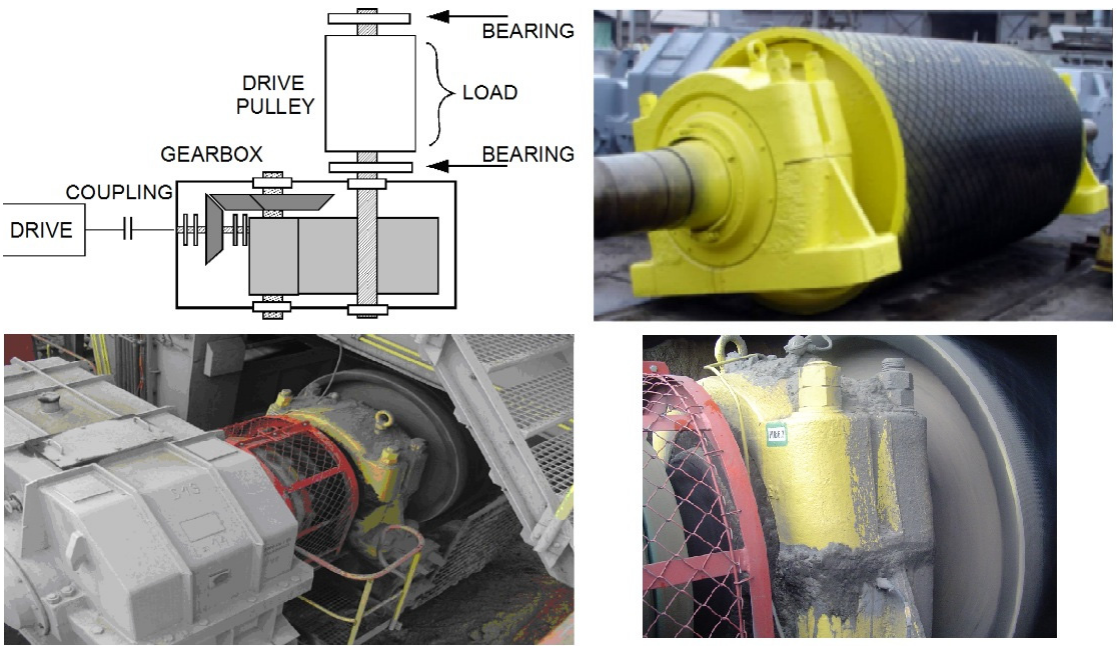
\includegraphics[width=0.9\textwidth]{gb.PNG}
\caption{The object of interest \label{f:rl}}
\end{center}
\end{figure}

\begin{figure}[!ht]
\begin{center}
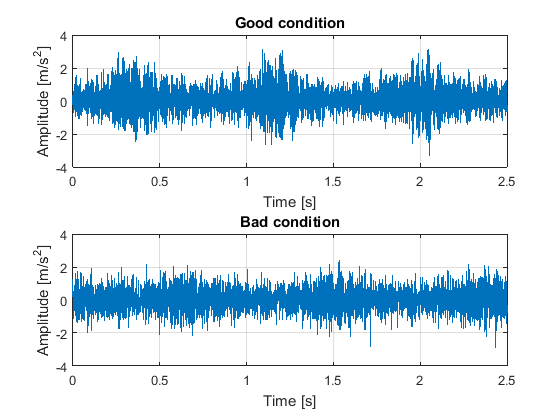
\includegraphics[width=0.8\textwidth]{fig2.png}
\caption{Raw vibration data \label{f:raw}}
\end{center}
\end{figure}

\begin{figure}[!ht]
\begin{center}
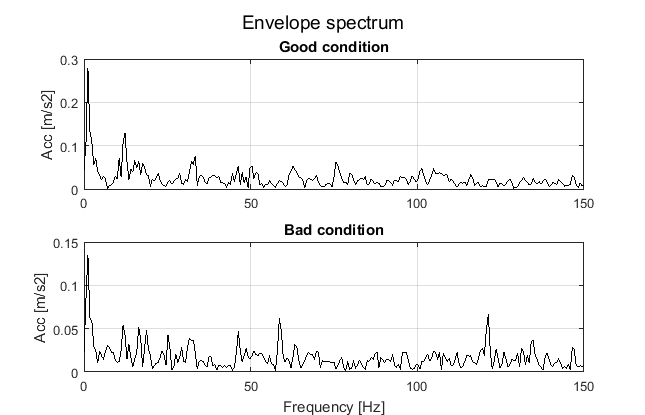
\includegraphics[width=0.8\textwidth]{envelope_raw.png}
\caption{Envelope spectrum of raw vibration data. \label{f:envelope_raw}}
\end{center}
\end{figure}

% \begin{figure}[!ht]
%   \centering
%   \begin{subfigure}[b]{0.48\textwidth}
%       \centering
% %  ?     \captionsetup{skip=0.01pt}
%   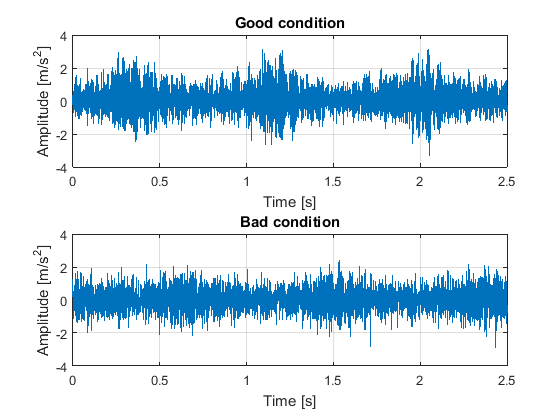
\includegraphics[width=1\textwidth]{fig2.png}
% \caption{Raw vibration data \label{f:raw}}
%   \end{subfigure}
%   %\hfill
%   \begin{subfigure}[b]{0.48\textwidth}
%       \centering
%     %   \captionsetup{skip=0.01pt}
% 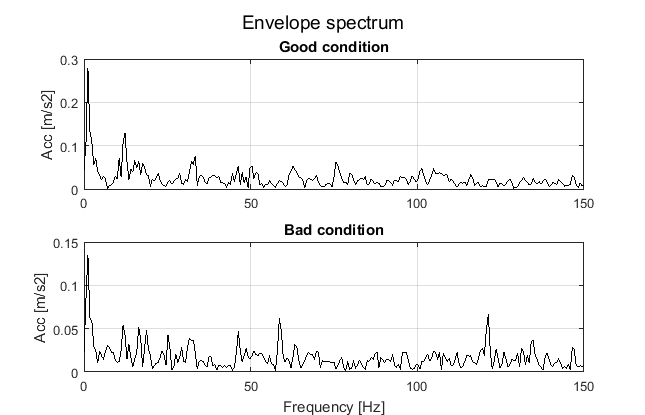
\includegraphics[width=1\textwidth]{envelope_raw.png}
% \caption{Envelope spectrum of raw vibration data. \label{f:envelope_raw}}
%   \end{subfigure}
%   \caption{One-dimensional sample variance of filtered AD map thresholded by local minimum of smoothed histogram of the variance vector}
%   \label{fig:fig_razem}
% \end{figure}

In Figure \ref{f:envelope_raw} we present the envelope spectrum of both analyzed signals. As one can notice, it is difficult to observe the impulsive behavior of the signal corresponding to machine in bad condition. The envelope spectrum also does not give the clear message about the damage. 



In Figure \ref{f:spec1} we present the  time-frequency representation (spectrogram) of signals from Figure \ref{f:raw}. They were calculated according to parameters in Table \ref{tab:tab}. On the spectrogram corresponding to signal from the machine in bad condition, we observe peaks between around 1 to 6 kHz. 


\begin{figure}[!ht]
\begin{center}
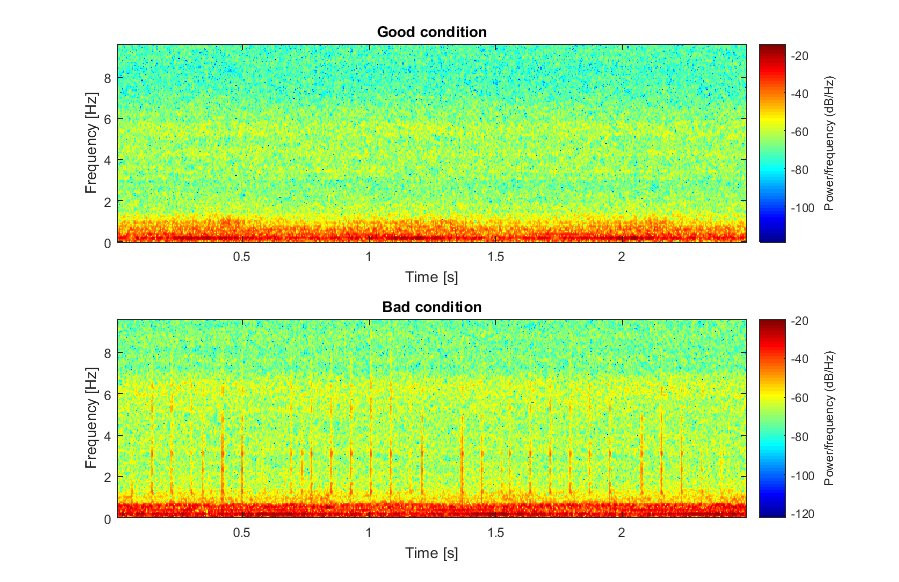
\includegraphics[width=0.8\textwidth]{spec.png}
\caption{Time-frequency representation (spectrogram) of the input data. \label{f:spec1}}
\end{center}
\end{figure}


\begin{table}[ht!]
    \centering
    \caption{Parameters of compared results.}
  \begin{tabular}{|l|l|}
    \hline
    \textbf{Parameter} & \textbf{Value} \\ \hline
         Sampling frequency & 19200 Hz \\ \hline
         Window & Hamming, 256 samples \\ \hline
         Overlap & $60\%$ window \\ \hline
         FFT points & 512 \\
    \hline
    \end{tabular}
    \label{tab:tab}
\end{table}

Next, the ADF statistic for each frequency bin from the spectrogram was calculated. In Figure \ref{f:stats} the values of ADF statistic are presented. For those frequencies for which we expect the impulsive behavior, the values of the statistic are lower. This indicates the subsignals corresponding to those frequencies are "more nonstationary" than for the other frequency bands.

\begin{figure}[!ht]
\begin{center}
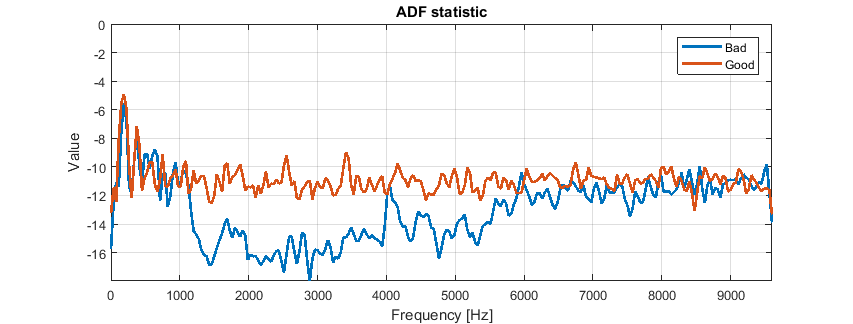
\includegraphics[width=0.8\textwidth]{lozysko_stats1_2.png}
\caption{ADF statistic  for signal of the machine in good and bad condition. \label{f:stats}}
\end{center}
\end{figure}

In Figure \ref{f:selector} we present the ADF selector, i.e. the absolute value of the ADF statistic and the corresponding filter characteristic.

\begin{figure}[!ht]
\begin{center}
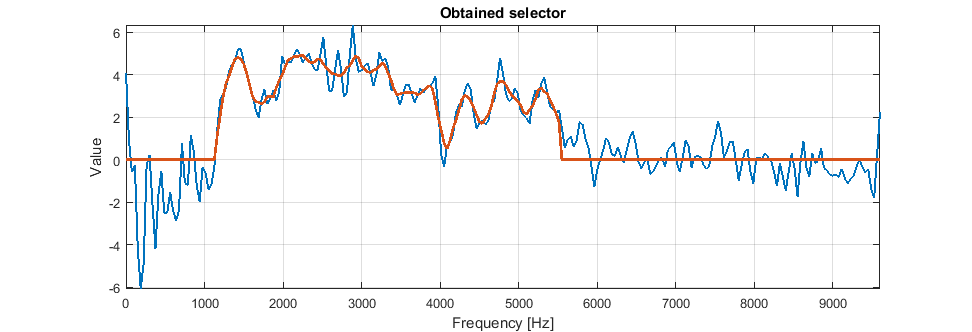
\includegraphics[width=0.8\textwidth]{selector_3.png}
\caption{ADF selector and ADF filter characteristic.\label{f:selector}}
\end{center}
\end{figure}

After filter function is obtained, next step is the signal filtration. In Figure \ref{f:filtered} we present the signal from the machine in bad condition filtered using obtained characteristics, while in Figure \ref{f:spec_filtered} shows the corresponding spectrogram of filtered signal.



\begin{figure}[!ht]
  \centering
  \begin{subfigure}[b]{0.7\textwidth}
      \centering
%  ?     \captionsetup{skip=0.01pt}
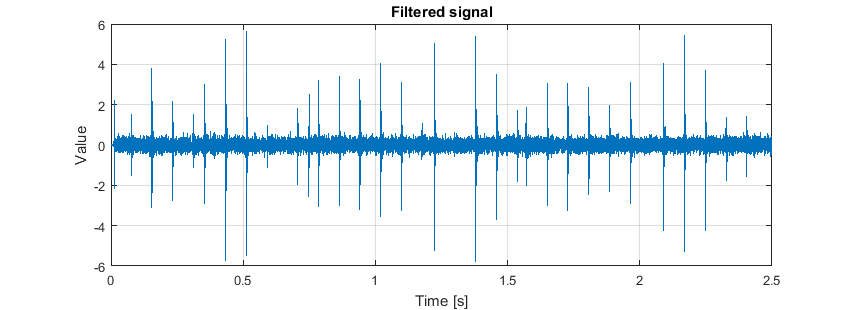
\includegraphics[width=\textwidth]{filtered_signal_2.png}
\caption{Signal after filtration using ADF filter characteristic. \label{f:filtered}}
  \end{subfigure}
  %\hfill
  \begin{subfigure}[b]{0.7\textwidth}
      \centering
    %   \captionsetup{skip=0.01pt}
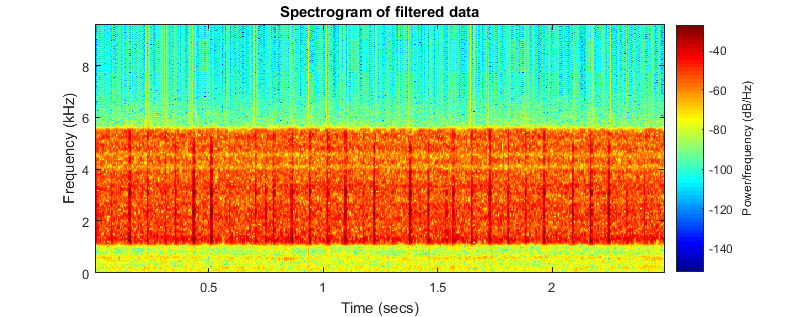
\includegraphics[width=\textwidth]{spec2_1.png}
\caption{Spectrogram of filtered signal. \label{f:spec_filtered}}
  \end{subfigure}
  
    \begin{subfigure}[b]{0.7\textwidth}
      \centering
    %   \captionsetup{skip=0.01pt}
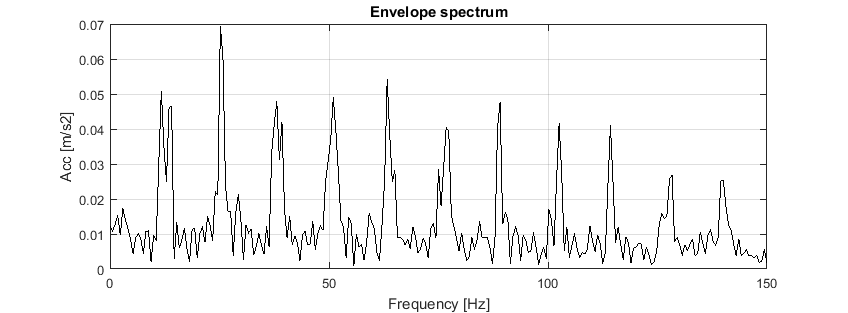
\includegraphics[width=\textwidth]{envelope_2.png}
\caption{Envelope spectrum of filtered signal. \label{f:envelope}}
  \end{subfigure}
  \caption{Presentation of signal in various domains after filtration procedure using obtain selector.}
  \label{fig:fig_razem}
\end{figure}




% \begin{figure}[!ht]
% \begin{center}
% 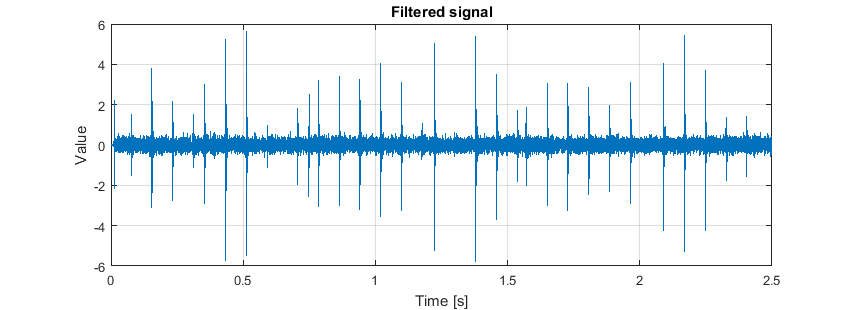
\includegraphics[width=0.8\textwidth]{filtered_signal_2.png}
% \caption{Signal after filtration using ADF filter characteristic. \label{f:filtered}}
% \end{center}
% \end{figure}

% \begin{figure}[!ht]
% \begin{center}
% 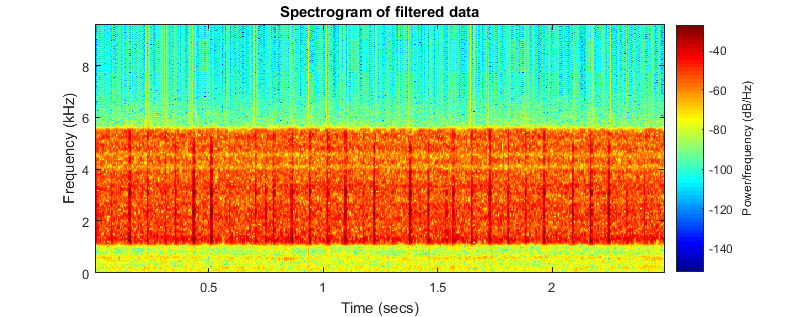
\includegraphics[width=0.8\textwidth]{spec2_1.png}
% \caption{Spectrogram of filtered signal. \label{f:spec_filtered}}
% \end{center}
% \end{figure}

% \begin{figure}[!ht]
% \begin{center}
% 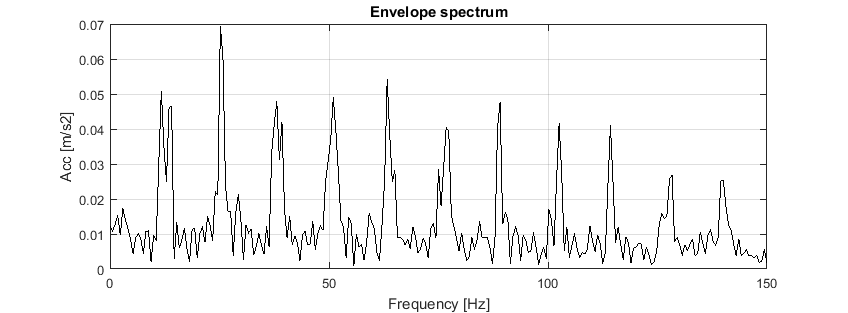
\includegraphics[width=0.8\textwidth]{envelope_2.png}
% \caption{Envelope spectrum of filtered signal. \label{f:envelope}}
% \end{center}
% \end{figure}



Finally we analyze the envelope spectrum of the filtered signal. As one can observe, the impulsiveness is easier to detect than for the original signal, for comparison see Figure \ref{f:envelope_raw} and Figure \ref{f:envelope}.
In order to compare SK- and ADF- selector results we have applied similar methodology for SK approach. More precisely, for the raw signal corresponding to the machine in bad condition, we calculated the SK and filtered the signal according to SK characteristic.  Similar as for ADF statistic, the SK statistic was also smoothed and thresholded (see the red line in Figure \ref{f:SK}). Finally we compared the kurtosis of the envelope of the filtered signals obtained after using ADF and SK approach.  The kurtosis of the envelope of filtered data  for ADF selector is 88.2290 while  for SK - 66.7322.

\begin{figure}[!ht]
\begin{center}
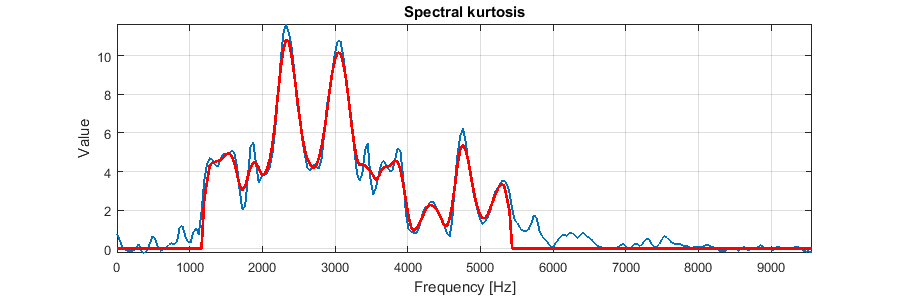
\includegraphics[width=0.8\textwidth]{SK2.png}
\caption{Spectral kurtosis and SK selector. \label{f:SK}}
\end{center}
\end{figure}


\section{Conclusions}
The approach presented in this paper is a continuation of the authors previous work, where number of IFB selectors was proposed. However a classical approach was described by Antoni and Randall, who indicated the spectral kurtosis as the proper measure of impulsiveness and therefore the effective IFB selector. Our approach is based on the calculating how nonstationary is the analyzed signal. We proposed the ADF statistic as the measure of nonstationarity which follows from the impulsive behavior of the signal in IFB. We have described the proposed procedure in which the final step is the filtered signal according to the obtained signal characteristic. The resuls we have compared with the classical approach based on the SK and indicated that for the analyzed real signal the new algorithm is more effective than the algorithm based on the SK.


\bibliographystyle{ISMA}
\bibliography{mybibfile}

\end{document}
